\documentclass{standalone}
\usepackage{tikz}
\pagestyle{empty}
\usetikzlibrary{positioning}

\begin{document}
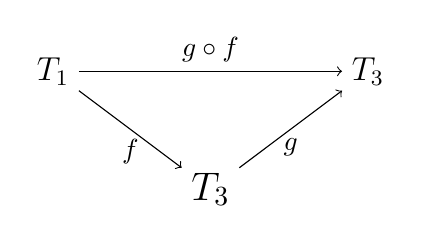
\begin{tikzpicture}
  \begin{scope}[on grid, node distance=4cm]

  \node (m-1-1) at (0,0) {\large $T_1$};
  \node[right=of m-1-1] (m-1-3) {\large $T_3$};
  \node[below right= 1.5cm and 2cm of m-1-1] (m-2-2) {\Large $T_3$};

  \path[->,font=\normalsize]
  (m-1-1) edge                node[above] {$g\circ f    $} (m-1-3);
  \path[->,font=\normalsize]
  (m-1-1) edge                node[below] {$f           $} (m-2-2);
  \path[->,font=\normalsize]
  (m-2-2) edge                node[below] {$g           $} (m-1-3);

  \end{scope}
\end{tikzpicture}
\end{document}
